% Proposta B (12/11/2026, pedido do autor): a mesma integração da proposta A,
% 12/11/2026, pedido do autor: entrada "Série de preços" e as duas perguntas.
% com as duas maneiras de usar a volatilidade prevista (filtro e ajuste da
% posição) da subseção "Uso da volatilidade prevista na operação" do Cap. I.
% Mostra as duas combinadas, como o último parágrafo da subseção descreve (o
% filtro veta, e nos dias liberados a posição é menor quanto maior a
% volatilidade). Mesmo estilo das fig05/fig06. Fora do TG até o autor decidir.
\documentclass[11pt,border=2pt]{standalone}
\usepackage[T1]{fontenc}
\usepackage[utf8]{inputenc}
\usepackage{mathptmx}
\usepackage{tikz}
\usetikzlibrary{arrows.meta,positioning,calc,shapes.geometric}
\tikzset{
  seta/.style={-{Stealth[length=2.2mm]}, semithick},
  caixa/.style={rectangle, draw, semithick, fill=gray!10, rounded corners=2pt,
                align=center, minimum width=46mm, minimum height=10mm, font=\small},
  dado/.style={trapezium, trapezium left angle=75, trapezium right angle=105, draw,
               semithick, fill=white, align=center, minimum height=9mm, font=\small,
               trapezium stretches body},
  decisao/.style={diamond, draw, semithick, fill=white, aspect=2.4, align=center,
                  inner sep=1pt, font=\small},
  rotulo/.style={font=\footnotesize\itshape, align=center},
}
\begin{document}
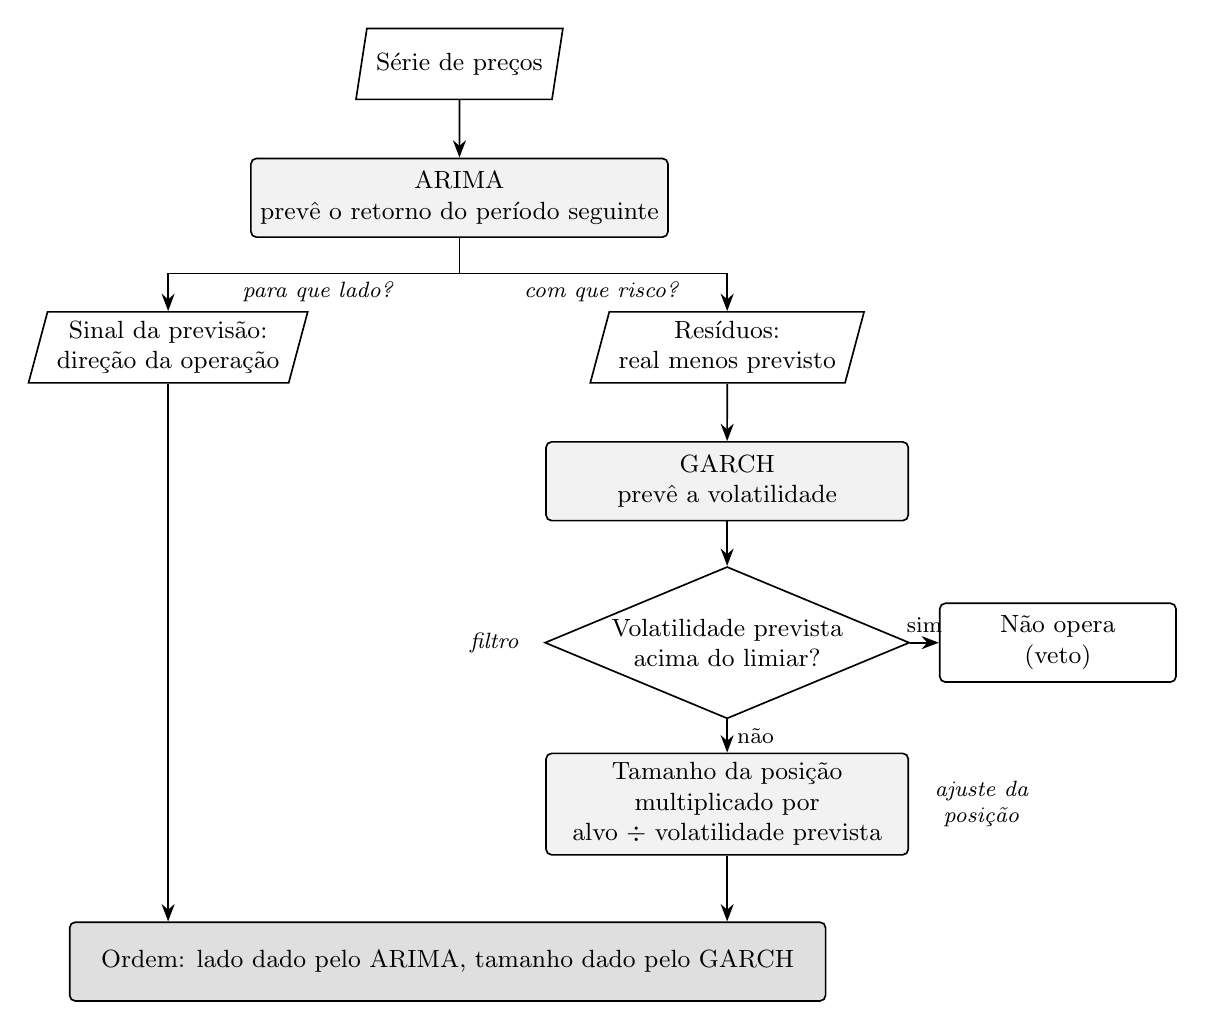
\begin{tikzpicture}
  \node[dado] (ent) at (0,0) {Série de preços};
  \node[caixa] (arima) at (0,-1.7) {ARIMA\\prevê o retorno do período seguinte};

  \node[dado] (dir) at (-3.7,-3.6) {Sinal da previsão:\\direção da operação};
  \node[dado] (res) at (3.4,-3.6) {Resíduos:\\real menos previsto};
  \node[caixa] (garch) at (3.4,-5.3) {GARCH\\prevê a volatilidade};
  \node[decisao] (lim) at (3.4,-7.35) {Volatilidade prevista\\acima do limiar?};
  \node[caixa, minimum width=30mm, fill=white] (veto) at (7.6,-7.35) {Não opera\\(veto)};
  \node[caixa] (tam) at (3.4,-9.4) {Tamanho da posição\\multiplicado por\\alvo $\div$ volatilidade prevista};

  \node[caixa, minimum width=96mm, fill=gray!25] (ord) at (-0.15,-11.4)
    {Ordem: lado dado pelo ARIMA, tamanho dado pelo GARCH};

  \draw[seta] (ent) -- (arima);
  \draw[seta] (arima.south) -- ++(0,-0.45) -| (dir.north);
  \draw[seta] (arima.south) -- ++(0,-0.45) -| (res.north);
  \draw[seta] (res) -- (garch);
  \draw[seta] (garch) -- (lim);
  \draw[seta] (lim) -- node[above, font=\footnotesize]{sim} (veto);
  \draw[seta] (lim) -- node[right, font=\footnotesize]{não} (tam);
  \draw[seta] (tam.south) -- (tam.south |- ord.north);
  \draw[seta] (dir.south) -- (dir.south |- ord.north);

  \node[rotulo, anchor=east] at ([xshift=-2mm]lim.west) {filtro};
  \node[rotulo, anchor=west] at ([xshift=2mm]tam.east) {ajuste da\\posição};
  % as duas perguntas que a integração separa (Cap. I, 2º parágrafo da seção)
  \node[rotulo, below] at (-1.8,-2.65) {para que lado?};
  \node[rotulo, below] at (1.8,-2.65) {com que risco?};
\end{tikzpicture}
\end{document}
